\documentclass[12pt]{elsarticle}
\usepackage{amsmath}
\usepackage{pgfplots,tikz,graphicx,array}
\usepackage[margin=1.2in]{geometry}



\begin{document}

\begin{frontmatter}
\title{Optimization of a schedule-free water-bus system with autonomous vessels}

\begin{abstract}
In this talk we consider using autonomous vessels for transporting people
on the coastal area of a small city. Typically, vessels are schedule with
predefined arrival and departure times established by the management
following some criteria or a model. We propose an approach aiming to
enhance the system operation, moving from a full fixed schedule to a system
that follows the demand. We propose an optimization model aiming to
minimize the penalty assigned to the deviation from the targeted users’
arrival times. One challenge is that including full flexibility on the
schedule may lead to problems that are impractical due the time required to
find a solution, hence, defeating the purpose of an approach that aims to
follow demand. To overcome that challenge, we developed an optimization
model that mixes  typical patterns of passenger movements for some
established boat routes, while reserving some of the system capacity to
respond to the dynamics of the demand. While the system could be in
principle implemented with manned boats, the uncertainty introduced by the
demand response schedule may lead to confusion and errors by the crew, and
also not be incompatible with labor agreements. For that reason, the use of
autonomous vessels is key to respond more precisely to last minute changes
to the stops schedule. We present some illustrative examples to show that
the schedules found with this approach are both practical and may lead to a
more efficient and flexible use of the boats in peak hours.
\end{abstract}
\end{frontmatter}

Cite our survey \cite{Gu2021}

-----------------

Water-bus in Zhoushan city, hub and spoke design. \cite{Yu2015}

-----------------

When demand densities differ considerably over time or space, mixed fleets
can reduce total system cost compared to single fleets because vehicles of
different sizes may be attached to the operations for which they are most
suited. \cite{Kim2013}

-----------------

Mixing vehicle sizes \cite{Sun2015}

-----------------

High-frequency transport operations are affected by stochasticity on running
times and demand that usually lead to significant differences between planned
schedules and delivery. Research has shown that the most effective control
strategies do not adhere to schedules but aim for headway regularity and
passenger cost minimization. Operating high-frequency transit without
schedule is enable by passengers' unawareness of schedules and recent
advances in information technology. Passengers in this systems do not plan to
take a specific schedule vehicle but to wait a short time after their arrival
at a stop. Current best practices is to produce schedules in the planning
phase and subsequently ignore of abandon them in the service deliver phase to
deal with disruptions. Under the schedule based approach the operations plan
is fully defined, and therefore fixed, before service delivery. This involves
timetable development and vehicle and crew scheduling. Crew scheduling
assigns sets of vehicle trips to drivers in accordance with work rules
governing shift duration, breaks, and pay povisions.

A critical aspect of schedule-free operations is that potential performance
benefits can only be realized if a successful optimization approach exist.
 \cite{Sanchez2017}.

------------------

One of the main factors that affects the passengers satisfaction is their
travel and waiting time. Also, unpredicted variations in passenger flow is
one of the main sources of dissatisfaction. A multi-objective optimization
model for robust skip-stop scheduling with earliness and tardiness penalties.
\cite{Rajabighamchi2019}

Technological improvements have played a key role in the development of
public transportation system to make them both more effective and more
efficient. Information technologies are a key component to improve the
quality of service delivered to the users \cite{Hidalgo2014}. This has been
the case for both busses and train based systems
\cite{Hidalgo2014,Rajabighamchi2019}.



Information technologies play a major role in advance planning and control of
the systems due to its intrinsic complexity. Planning involves defining the
routes and scheduling the buses and crews.\cite{Hidalgo2014}

Bus and crew scheduling has been one of the most studied issues in transit
operations planning as they represent most of the costs of transit operators.
Many transit agencies and operators have developed software based on linear
programming algorithms. The use of the advance software has helped to
significantly reduce turnaround time in preparing buses and driver schedules,
distribute more evenly the personnel, and reduce operational
costs.\cite{Hidalgo2014}

Advance systems typically integrate elements such as information technology
applications for centralized control and combined service plans according to
the passengers demand characteristics.

\section{Description}

In this paper we consider a high frequency service water-bus system design
for a small coastal city. We define this as a high-frequency service because
the users waiting time to board a water bus will not have exceed 15 minutes
at any stop. We consider a city with several stops in the coastal area and a
fleet of vessels to serve the demand. Typically, in a high frequency system
there is a schedule with predefined arrival and departure times established
by the management following some criteria or a model. We propose an approach
aiming to enhance the system operation, moving from a full fixed schedule to
a system that follows the demand.

To follow the demand, we assume the existence of an information system that
allows the users to state a desired destination and arrival time. The goal is
to use the potential that modern information systems provide to lead the
system to respond to the users needs, and not the other way around. The users
preferences are then use to define a penalization that will discourage the
deviation from the user preferences when the routing of the vessels is
defined. For the sake of efficiency in the routing calculation, we will take
into consideration major patterns that is frequently found in the users
requirements. That allows as to fix some main routing connections.

One challenge is that including full flexibility on the schedule may lead to
problems and solution approaches that are impractical due the time required
to find a solution. hence, defeating the purpose of an approach that aims to
follow demand. To overcome that challenge, we developed an optimization model
that mixes typical patterns of passenger movements for some established boat
routes, while reserving some of the system capacity to respond to the
dynamics of the demand.

A major contribution of this work is to consider the use of autonomous
vessels. While the system could be in principle implemented with manned
boats, the uncertainty introduced by the demand response schedule may lead to
confusion and errors by the crew, together with requirements conflicting with
labor agreements. For that reason, the use of autonomous vessels is key to
respond more precisely to last minute changes to the stops schedule.


%an autonomous vessel that is transporting people between points $A$ and $B$
%in a city. For example, a boat traveling between Ask{\o}y and Bergen city
%center.  The typical schedule of a boat having stops $\ell \in \{A,B\}$ in
%this situation has some given arrival times, $a_{0,\ell}, a_{1,\ell}, \dots,
%a_{n,\ell}$ and departure times $d_{i,\ell}, \dots, d_{n,\ell}$ where, $i \in
%\{0,\dots,n\}$ is the i\textsuperscript{th} trip to $\ell$, this may be
%established by the management of the system following some criteria or may be
%determined by a model. Assume initially that the travel times $t_{A,B}$ and
%$t_{B,A}$, are regular and deterministic, which would lead to deterministic
%arrival times once the departure times are decided.
%
%This situation is illustrated in Figure
%\ref{fig:ABschedule}.
%
%\begin{figure}[h]
%  \centering
%  \begin{tikzpicture}[node distance=2.5cm]
%    \node at (-0.5, 0.4) (Atime0a) {$a_{0,A}$};
%    \node at (0.5, 0.4) (Atime0d) {$d_{0,A}$};
%    \node at (2.0, 0.4)(Btime0a)  {$a_{0,B}$};
%    \node at (3.0, 0.4) (Btime0d) {$d_{0,B}$};
%    \node at (4.5, 0.4)(Atime1a) {$a_{1,A}$};
%    \node at (5.5, 0.4)(Atime1d) {$d_{1,A}$};
%    \node at (7.0, 0.4)(Btime1a) {$a_{1,B}$};
%    \node at (8.0, 0.4)(Btime1d) {$d_{1,B}$};
%    \node at (12.0, 0.4)(Btime1d) {$a_{n,A}$};
%
%
%    \draw node at (0, 0) (A1) {$A$}
%    node (B1) [right of=A1] {$B$}
%    node (A2) [right of=B1] {$A$}
%    node (B2) [right of=A2] {$B$}
%    node (dots) [right of=B2] {$\dots$}
%    node (An) [right of=dots] {$A$};
%
%    \draw[->] (A1) -- (B1) node[midway,below]{$t_{A,B}$};
%    \draw[->] (B1) -- (A2) node[midway,below]{$t_{B,A}$};
%    \draw[->] (A2) -- (B2) node[midway,below]{$t_{A,B}$};
%    \draw[->] (B2) -- (dots) node[midway,below]{$t_{B,A}$};
%    \draw[->] (dots) -- (An) node[midway,below]{$t_{B,A}$};
%  \end{tikzpicture}
%  \caption[two points case]{Typical schedule for a two point
%    transport}
%  \label{fig:ABschedule}
%\end{figure}
%
%\subsection{Flexible times schedule}
%
%For our first approach to a flexible schedule, we consider the
%preferred arrival time $f^p _ {\ell}$ for each passenger $p$ who want
%to travel to $\ell \in \{A, B\}$. Also, for each passenger (this could
%be a group of passengers as well) we use the following penalization
%parameters for deviations from the preferred arrival time
%$f^p _ {\ell}$:
%\begin{itemize}
%\item let $\alpha^p_{\ell}$ the penalization term for arrivals earlier
%  than desired time, i.e., when $f^p _ {\ell} - a_{i,\ell} > 0$;
%\item let $\beta^p_{\ell}$ the penalization term for arrival later
%  than desired time: $f^p _ {i,\ell} - a_{i,\ell} < 0$.
%\end{itemize}
%
%The $\alpha^p_{\ell}$ penalties could be interpreted as a big fixed
%cost (missing a connecting transport to another location) plus a
%smaller linear variable cost. Early arrival $\beta^p_{\ell}$ penalties
%could be assumed as linear.
%
%Using these penalties, the goal is to find a schedule for departure
%times $d_{i,\ell}$, $i \in \{0,\dots,n\}$ and $\ell \in \{A,B\}$, such
%that it will minimize the total penalty over all users. Recall the
%assumption of deterministic travel times. Another approach may be to
%minimize the sum $T + W$, where $T$ is traveling time and $W$ is the
%waiting time at the stops.
%\\*It is important to note that it is assumed the passenger would take
%the ferry most suitable to them according to the timetable which in
%turn is according to the input given by the passengers.\\*
%
%
%\subsection{A system with two vessels}
%
%A generalization of our model is to consider two vessels in the
%system. In particular, fixed scheduling of two boats are usually done
%such that the boats are simultaneously departing from opposite ends of
%the route. A fixed schedule like this may lead to sub-utilization of
%one of the boats during a rush hour. The case is illustrated in Figure
%\ref{fig:towVFixSch}. An example of this situation is the operation of
%two ferries in a river crossing.
%
%\begin{figure}[h]
%  \centering
%  \begin{tikzpicture}
%
%    \draw node (A) at (-4, 0.5) {\large A} %%
%    node (WaitingA) at (-4.2, 1.5)
%    {\includegraphics[width=.1\textwidth]{PeopleWaiting.jpg}} %%
%    node (B) at (4, 0.5) {\huge B};
%
%    \draw node (right) at (0,0)
%    {\includegraphics[width=.12\textwidth]{Rowboat.jpg}};
%
%    \draw node (left) at (0,1)
%    {\scalebox{-1}[1]{\includegraphics[width=.12\textwidth]{RowboatL.jpg}}};
%
%    \draw[->] (A) -- (right);
%    \draw[->] (left) -- (A);
%    \draw[->] (right) -- (B);
%    \draw[->] (B) -- (left);
%
%  \end{tikzpicture}
%  \caption{Two vessels with fixed schedule}\label{fig:towVFixSch}
%\end{figure}
%
%The aim of a flexible schedule, is the effective utilization of the
%ferry specially during peak hour. The schedule would change
%dynamically if arrival times are allowed to respond to the users
%arrival expectations. Consider again the case in Figure
%\ref{fig:towVFixSch}. With a flexible schedule it would be possible
%that both vessels would be departing one after the other to the same
%end on a rush hour, as is illustrated in Figure
%\ref{fig:towVFlex}. Ideally, this would reduce the waiting time for
%the passengers at the most crowded. However, the solution is not
%trivial. In particular, if the demand is much higher than the capacity
%of the two boats, the waiting time would be the whole round trip of
%the two boats. Hence, the aim of a flexible schedule is to consider
%the right criteria to improve the service level of the system. Here,
%the service level has to be defined appropriately.
%
%\begin{figure}[h]
%  \centering
%  \begin{tikzpicture}
%
%    \draw node (A) at (-4, 0.5) {\large A} %%
%    node (WaitingA) at (-4.2, 1.5)
%    {\includegraphics[width=.1\textwidth]{PeopleWaiting.jpg}} %%
%    node (B) at (4, 0.5) {\huge B};
%
%    \draw node (right) at (-2.8,0)
%    {\includegraphics[width=.12\textwidth]{Rowboat.jpg}};
%
%    \draw node (left) at (-2.8,1)
%    {\includegraphics[width=.12\textwidth]{RowboatL.jpg}};
%
%    \draw[->] (right) -- (B);
%    \draw[->]  (left) -- (B);
%
%  \end{tikzpicture}
%  \caption{Two vessels with fixed schedule}\label{fig:towVFlex}
%\end{figure}
%
%The aim is to generalize this problem to consider $n$ vessels in the
%system, with more than two stops and a mixed fleet of
%autonomous and manned vessels. The mixed fleet may help to find the
%right balance among the different demands during the day. For example,
%the autonomous vessels could be used late at night to serve the low
%demand.



\section{Optimization of the Schedule free operational plan}

The system underlying our model is a water-bus system with a set of stops
$\mathcal{S}$ and a set of identical vessels $\mathcal{V}$. To obtain a
schedule free optimized routing we do not aim to obtain a fixed schedule for
the operation of the vessels. Instead, we will rout the vessels to obtain an
operational plan that will minimize the total cost for the passengers. To
measure that cost we penalize the deviation of the arrival times obtain with
the operational plan from the desired arrival times stated by the passengers.

Hence, we consider a set of passengers $\mathcal{P}$ that will be assigned to
a particular vessel. To handle the lack of preassigned routes we will use a
set of vessel hops $\mathcal{H}$. Here a hop is defined as the movement of a
vessel between to arbitrary stops. Note that the maximum number of hops can
be bounded dividing the length of a time horizon by the time duration of the
shortest hop. Also, a single vessel may no used all the hops it is allowed to
use within a particular time horizon. We summarize the sets and parameters
defined for the model in table \ref{tab:parameters}
\begin{table}
  \centering
  \begin{tabular}{ll}
  \hline
  $\mathcal{S}$ &  Set of stops \\
  $\mathcal{V}$ &  Set of vessels \\
  $\mathcal{P}$ & Set of passengers\\
  $\mathcal{H}$ & Set of possible vessel hops\\
  $T$ & Time horizon \\
  $\beta_{p}$ & Penalization rate for late arrival than desired
                   for a passenger $p$ \\
  $\alpha_{p}$ & Penalization rate for early arrival than desired
                 for a passenger $p$ \\
  $t_{ij}$ & Travel time for a vessel from $i$ to $j$, $i \neq j$ \\
  $f_p$ & Preferred arrival time for passenger $p$.\\
  $s_p$ & Stop for passenger $p$.\\
  $o_p$ & Origin for passenger $p$.\\
  $r$ & The cost rate per unit of time for a vessel hope.\\
  \hline
\end{tabular}
  \caption{Sets and parameters for the operational optimization}\label{tab:parameters}
\end{table}

We assume that the passengers targeted arrival times is information available
in an online system used by the passengers. The input of this demand makes it
possible to optimize the operational plan. In addition, we assume that the
passengers will be travelling using the optimized assignments. Henceforth,
the operational plan needs to define an assignment of passengers $p \in
\mathcal{P}$ to particular vessels $i \in \mathcal{V}$ during one of their
hops $j \in \mathcal{H}$. For these decisions we define the following binary
variables:
\begin{equation}\label{eq:passengerAssignment}
    x_{vhij} = \begin{cases}
                 1, & \mbox{if vessel $v$ in its $h$ hop travels from stop $i$ to stop $j$}\\
                 0, & \mbox{otherwise}.
               \end{cases}
\end{equation}

Additionally, we need to route the vessels $i \in \mathcal{V}$ defining the
stops $s \in \mathcal{S}$ to depart and arrive in each hop $j \in
\mathcal{H}$. For these decisions we define the following binary variables:
\begin{equation}\label{eq:passengerAssignment}
  y_{pvh} = \begin{cases}
    1, & \mbox{if passenger $p$ arrives to the destination traveling in vessel $v$ in its $h$ hop}\\
    0, & \mbox{otherwise}.
  \end{cases}
\end{equation}

\begin{equation}\label{eq:passengerAssignment}
  z_{pvh} = \begin{cases}
    1, & \mbox{if passenger $p$ boards at the origin traveling in vessel $v$ in its $h$ hop}\\
    0, & \mbox{otherwise}.
  \end{cases}
\end{equation}

             

Using the assignment variables we may compute the arrival times $a_{vh}$ for
vessel $v$ after hop $h$, and the arrival time $r_p$, earliness $e_p$, and
tardiness$d_p$ for passengers $p \in \mathcal{P}$.


\subsection{Mathematical Model}

\subsubsection{Objective function}

The objective function of the model is to minimize the total penalization for
missing the targeted arrival times over all the passengers define in
\eqref{eq:penalty}. There, we add the penalties for tardiness and earliness
obtained with the optimize operational plan.
\begin{equation}
  \sum_{p \in P} (\alpha_p e_p + \beta_p d_p) \label{eq:penalty}
\end{equation}
However, using these penalties alone may result in solutions where spurious
hops for the vessels are defined. Consider for example the case of a system
with a fleet of three vessels where only two are required to be routed within
some time horizon. If the hops of the vessels are costless the result is a
set of alternative optimal solutions where the unused vessel can hope freely
without penalizing the objective function. To avoid those spurious solutions
we introduce the hop cost using the cost rate $c$, which lead to the
objective function \eqref{eq:objective}. Notice that the objective function
gives a overall system cost. However, the emphasis in this model is on the
passengers cost.
\begin{equation}
  \min \ \sum_{p \in P} (\alpha_p e_p + \beta_p d_p) +
  \sum_{v \in \mathcal{V}} \sum_{h \in \mathcal{H}} \sum_{i \in \mathcal{S}} \sum_{j \in \mathcal{S}\setminus i} rt_{ij}x_{vhij}\label{eq:objective}
\end{equation}

\subsubsection{Constraints}

Nest, we need to ensure that the passengers can embark and disembark the
vessel there are assigned for their trip. To define the boundaries of the
feasible set of feasible operational plans we consider the following factors.

First, we need to ensure that all passengers are picked up at their origins
and deliver to their destinations. Hence, we first ensure that every
passenger embarks on a vessel to travel to the selected destination. We
achieve that with the set of constraints \eqref{eq:embark}, where we enforce
that a passenger is assigned to one vessel exclusively.
\begin{equation}
  \label{eq:embark}
  \sum_{v \in \mathcal{V}}  \sum_{h \in \mathcal{H}}^{T} y_{pvh} = 1 \;\forall p \in \mathcal{P}.
\end{equation}

\begin{equation}
  \label{eq:embark}
  \sum_{v \in \mathcal{V}}  \sum_{h \in \mathcal{H}}^{T} z_{pvh} = 1 \;\forall p \in \mathcal{P}.
\end{equation}

Then, we ensure that all passengers can disembark at their destination with
the set of constraints \eqref{eq:disembark}

\begin{equation}
  \label{eq:disembark}
  y_{pvh} \leq \sum_{i \in \mathcal{S}  \setminus s_p} x_{vhis_p} \;
  \forall p \in \mathcal{P}, v \in \mathcal{V},  h \in \mathcal{H}
\end{equation}

The boat a passenger boards has to stop at the passenger's
origin:

\begin{equation}
  \label{eq:stoporgn}
  z_{pvh} \leq \sum_{j \in \mathcal{S}  \setminus o_p}
  x_{vho_pj} \; \forall p \in \mathcal{P},  v \in
  \mathcal{V}, \bar h \in \mathcal{H}
\end{equation}

\begin{equation}
  \label{eq:onetrip}
  y_{pv\bar h} \le \sum_{h = 1}^{\bar h}  z_{pvh}  \forall p \in \mathcal{P}, v \in \mathcal{V},  \bar h \in \mathcal{H}
\end{equation}


In one trip a boat can only move between two stations:

\begin{equation}
  \label{eq:onetrip}
  \sum_{i \in \mathcal{S}} \sum_{j \in \mathcal{S}} x_{vhij} \le 1 \;
  \forall v \in \mathcal{V},  h \in \mathcal{H}
\end{equation}

Determine the arrival time of a boat after a trip, here $a_{v0}$ is
zero for all boats:

\begin{equation}
  \label{eq:arrivaltimevessel}
  a_{vt} = a_{vt-1} + \sum_{i \in \mathcal{S}} \sum_{j \in
    \mathcal{S}\setminus i} t_{i,j}x_{vhij} \; \forall v \in
  \mathcal{V}, t \in \{1,\dots,T\}
\end{equation}

The arrival of a passenger, $M$ is the upper bound for arrival time:

\begin{equation}
  \label{eq:arrivaltimepassenger}
  r_p \ge a_{vt} - (1 - y_{pvh})M \; \forall p \in \mathcal{P}, v \in
  \mathcal{V}, t \in \{1,\dots,T\}
\end{equation}

\begin{equation}
  \label{eq:arrivaltimepassenger2}
  r_p \le a_{vh} + (1 - y_{pvh})M \; \forall p \in \mathcal{P}, v \in
  \mathcal{V}, t \in \{1,\dots,T\}
\end{equation}

Tardiness of a passenger:

\begin{equation}
  \label{eq:tardiness}
  d_p \ge r_p - f_p  \; \forall p \in \mathcal{P}
\end{equation}

Earliness of a passenger:

\begin{equation}
  \label{eq:tardiness}
  e_p \ge f_p - r_p  \; \forall p \in \mathcal{P}
\end{equation}

Connectivity of the schedule:

\begin{equation}
x_{vhij} \le \sum_{\ell \in S\setminus i} x_{vh-1\ell i} \; \forall v \in  \mathcal{V}, i,j \in \mathcal{S}, t \in \{2,\dots,T\}
\end{equation}

Non-negativity:

\begin{equation}
  \label{eq:nonnegativity}
  a_{vt}, r_p, d_p, e_p \ge 0 \; \forall p \in \mathcal{P}, v \in
  \mathcal{V}, t \in \{1,\dots,T\}
\end{equation}

Binary constraints:

\begin{equation}
  \label{eq:binary}
  x_{vhij}, y_{pvh} \in \{0,1\} \; \forall p \in \mathcal{P}, v \in
  \mathcal{V}, t \in \{1,\dots,T\}, i,j \in \mathcal{S}
\end{equation}

\section{Solution approach}

The planning problem can be decompose into a trip sequence problem and a
departure times subproblem. \cite{Sanchez2017}

\section{Results}
\begin{figure}[h]
  \centering
  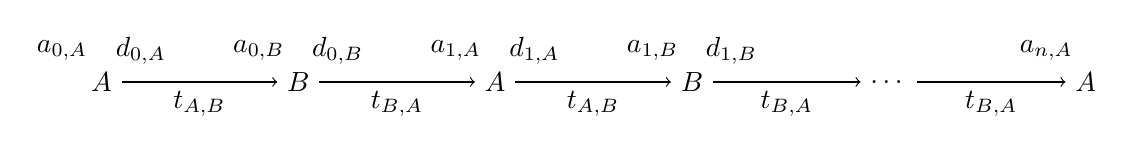
\begin{tikzpicture}[node distance=2.5cm]
    \node at (-0.5, 0.4) (Atime0a) {$a_{0,A}$};
    \node at (0.5, 0.4) (Atime0d) {$d_{0,A}$};
    \node at (2.0, 0.4)(Btime0a)  {$a_{0,B}$};
    \node at (3.0, 0.4) (Btime0d) {$d_{0,B}$};
    \node at (4.5, 0.4)(Atime1a) {$a_{1,A}$};
    \node at (5.5, 0.4)(Atime1d) {$d_{1,A}$};
    \node at (7.0, 0.4)(Btime1a) {$a_{1,B}$};
    \node at (8.0, 0.4)(Btime1d) {$d_{1,B}$};
    \node at (12.0, 0.4)(Btime1d) {$a_{n,A}$};


    \draw node at (0, 0) (A1) {$A$}
    node (B1) [right of=A1] {$B$}
    node (A2) [right of=B1] {$A$}
    node (B2) [right of=A2] {$B$}
    node (dots) [right of=B2] {$\dots$}
    node (An) [right of=dots] {$A$};

    \draw[->] (A1) -- (B1) node[midway,below]{$t_{A,B}$};
    \draw[->] (B1) -- (A2) node[midway,below]{$t_{B,A}$};
    \draw[->] (A2) -- (B2) node[midway,below]{$t_{A,B}$};
    \draw[->] (B2) -- (dots) node[midway,below]{$t_{B,A}$};
    \draw[->] (dots) -- (An) node[midway,below]{$t_{B,A}$};
  \end{tikzpicture}
  \caption[two points case]{Typical schedule for a two point
    transport}
  \label{fig:ABschedule}
\end{figure}

[[0, 2.8, 0, 1, 14.27],
[0, 4.64, 0, 1, 13.0],
[0, 6.0, 0, 1, 21.31],
[0, 2.45, 5, 1, 11.49],
[0, 8.16, 5, 2, 20.65],
[0, 4.12, 5, 1, 14.88],
[0, 6.16, 3, 1, 8.92],
[0, 6.89, 4, 2, 10.36],
[0, 5.62, 4, 2, 15.4],
[0, 6.26, 0, 1, 19.63]]

[[0, 2.8, 0, 1, 14.27],
[0, 4.64, 0, 1, 13.0],
[0, 6.0, 0, 1, 21.31],
[0, 2.45, 5, 1, 11.49],
[0, 8.16, 5, 2, 20.65],
[0, 4.12, 5, 1, 14.88],
[0, 6.16, 3, 1, 8.92],
[0, 6.89, 4, 2, 10.36],
[0, 5.62, 4, 2, 15.4],
[0, 6.26, 0, 1, 19.63],
[0, 8.7, 5, 2, 8.53],
[0, 3.11, 4, 1, 14.59]]

1370.67

\bibliography{refsblabybane}
\bibliographystyle{plain}


\end{document}
%%% Local Variables:
%%% mode: latex
%%% TeX-master: t
%%% End:
